% !TEX root = ../thesis.tex
\subsection{Abstract}
We investigate reactions between laser-cooled \ce{Be+} ions and room-temperature water molecules using an integrated ion trap and high-resolution time-of-flight mass spectrometer. This system allows simultaneous measurement of individual reaction rates that are resolved by reaction product. The rate coefficient of the \ce{Be+(^2S1/2) + H2O -> BeOH+ + H} reaction is measured for the first time and is found to be approximately two times smaller than predicted by an ion-dipole capture model. Zero-point-corrected quasi-classical trajectory calculations on a highly accurate potential energy surface for the ground electronic state reveal that the reaction is capture-dominated, but a submerged barrier in the product channel lowers the reactivity. Furthermore, laser excitation of the ions form the \ce{^2S1/2} ground state to the \ce{^2P3/2} state opens new reaction channels, and we report the rate and branching ratio of the \ce{Be+(^2P3/2) + H2O -> BeOH + H} and \ce{H2O} + Be reactions. The excited-state reactions are nonadiabatic in nature.

\subsubsection{Introduction}

Low-temperature reactions of simple ions with small molecules play a central role in astrochemical environments from interstellar clouds to cometary comae to planetary atmospheres, including that of Earth\cite{Agundez2013,Krasnopolsky2014}. The chemical evolution of interstellar molecular clouds ultimately yields the seedbed from which new stars and planets are born and the raw materials from which life likely developed. A firm understanding of the reaction rates for a host of elementary ion-molecule reactions is essential to accurately model these environments these environments. Techniques such as selected ion flow tubes (SIFTs)\cite{Adams1976}, guided ion beams\cite{Armentrout2002}, and supersonic flows (CRESU)\cite{Sims2002} have improved our empirical understanding of these processes; however, each has its own limitations.\cite{Smith2000,Snow2008} Theoretically, it has long been recognized that these ion-molecule reactions are often barrierless, and their rates are frequently described by capture models.\cite{Gioumousis1958a} However, recent studies have revealed that dynamical features can sometimes prevail,\cite{Lourderaj2008,Li2014,Carrascosa2017} in which case statistical treatments may not be accurate.\cite{Hase2014,Clary1990} Therefore, new experimental and theoretical efforts are needed to accurately address ion-molecule chemistry.

We have developed an approach, adapted from the ultracold ion community,\cite{Hudson2016,Tomza2017,Willitsch2012a} to study reactions of atomic ions with small molecules. Here we report the use of this approach to study the reaction of \ce{Be+} with gas=phase water for the first time. There have been very few experimental studies of gas-phase reactions between metal ions and water, especially at low temperature, despite their importance for metal ion chemistry in a range of environments.\cite{Highberger2001,Oppenheimer2002,VanDishoeck2013a}

Singly ionized beryllium is a particularly attractive metallic reactant to use for such studies because it is both theoretically tractable and experimentally highly controllable. The relatively simple electronic structure of this three-electron ion allows both highly accurate characterization of its electronic structure and laser cooling,\cite{Bollinger1985} and the low mass of \ce{Be+} lends itself to high motional frequencies as well as efficient sympathetic cooling of other chemically interesting atomic ions when employed in ion traps.\cite{Chen2014a,Roth2006,Larson1986,Schowalter2016} For the molecular reaction partner, \ce{H2O} is arguably the most important molecule in chemistry, and theoretical studies of its reactions with a single atom have been reported on full-dimensional potential energy surfaces (PESs).\cite{Li2013,Song2015,Ray2017,Li2015,Xiao2011} Thus this system of reagents provides an opportunity to perform a high-resolution comparison between experiments and theory for a molecule-ion system.

The apparatus employed here is shown in the Supporting Information (SI) (Figure S1). Laser ablation of metallic \ce{Be} is used to produce \ce{Be+} ions, which are trapped in a linear radio frequency Paul trap.\cite{Wolfgang1990} Laser cooling \cite{Wineland1979} is used to cool the translational motion of the ions, resulting in a Coulomb crystal of \ce{Be+} ions. Gaseous, room-temperature \ce{H2O} molecules are then introduced via a leak valve into the trapping region, where they react with the trapped ions. Charged products of the chemical reaction remain in the trap and are subsequently detected via an integrated time-of-flight mass spectromemter (TOFMS) recently developed by our group\cite{Schowalter2012,Schneider2014} and used to discover new species.\cite{Puri2017} The total reaction rate is measured by monitoring the decay of \ce{Be+} ion fluorescence, and the product branching ratios are extracted from the mass spectrum.

A key feature of this experiment is that by varying the detuning of the 313 nm laser used to cool the ions, the population in the excited \ce{1s^2 2p^1 ^2P3/2} and ground \ce{1s^2 2s^1 ^2S1/2} states can be controlled. Because the energy difference between the ground and excited states is 3.96 eV, several more product channels are open for the \ce{Be+(^2P3/2) + H2O} entrance channel. Using this system, we are able to measure the reaction rate and product branching ratio for these two entrance channels. We find that the ground-state channel, \ce{Be+(^2P3/2) + H2O}, exclusively produces \ce{BeOH+ + H}, whereas the excited-state channel, \ce{Be+(^2P3/2) + H2O}, also produces \ce{H2O+ + Be} with a yield of $~10\%$. Specifically, the reactions considered here are

\begin{align}
	\ce{Be+(^2S1/2) + H2O & -> BeOH+ + H} \label{r: Be(S)+H2O->BeOH} \\
	\ce{Be+(^2P3/2) + H2O & -> BeOH+ + H} \label{r: Be(P)+H2O->BeOH} \\
	\ce{Be+(^2P3/2) + H2O & -> H2O+ + Be} \label{r: Be(P)+H2O->H2O} \\
	\ce{H2O + H2O+ & -> H3O+ + OH} \label{r: H2O+H2O->H3O} \\
	\ce{Be+(^2P3/2) + H2O & -> BeH+ + O2} \label{r: Be(P)+H2O->BeH} \\
	\ce{BeH+ + H2O & -> BeOH+ + H2} \label{r: BeH+H2O->BeOH} \\
	\ce{Be+(^2P3/2) + H2O & -> BeO+ + H2} \label{r: Be(P)+H2O->BeO} \\
	\ce{BeO+ + H2O & -> BeOH+ + OH} \label{r: BeO+H2O->BeOH}
\end{align}

Because the translational energy of the laser-cooled \ce{Be+} ions is $<0.5$ K, the energy of the room-temperature water sets the reaction kinetic energy of \ce{Be+ + H2O} in the center of mass frame fo $~100$K. The internal state distribution of the \ce{H2O} is assumed to be given by the 300 K. Typical TOF traces (10 sample average) at reaction times $t=0$ and 70 s with 7 and 26\% relative \ce{Be+(^2P3/2)} state excitation are shown in Figure 1A,B, respectively. The fluorescence signal, which is used to determine the reaction time zero and normalize the initial ion number for the TOF, is monitored by the camera (ANDOR iXON3 EMCCD) in real time. At $t=0$ s, a large peak of $m/z=9$(\ce{Be+}) and a smaller one of $m/z=9$(\ce{BeOH+}) are evidenced in the TOF trace (blue line), which indicates that \ce{Be+} ions are the main species in the trap at $t=0$. The finite amount of \ce{BeOH+} at $t=0$ reflects the fact that reactions \cref{r: Be(S)+H2O->BeOH,r: Be(P)+H2O->BeOH,r: Be(P)+H2O->H2O,r: H2O+H2O->H3O,r: Be(P)+H2O->BeH,r: BeH+H2O->BeOH,r: Be(P)+H2O->BeO,r: BeO+H2O->BeOH} happen even during the loading process and that the mass filtering procedure is imperfect. At $t-70$ s, a $m/z=19$ peak emerges when more \ce{Be+} ions are excited to \ce{^2P3/2} state\todo{ref figure}, which we identify as \ce{H3O+} resulting from reactions \cref{r: Be(P)+H2O->H2O,r: H2O+H2O->H3O}. The \ce{BeOH+ / H3O+} ratio, $\eta(P_\text{P})$, is measured by integrating both peaks for the experimentally controlled excited-state population $P_\text{P}$. The \ce{BeOH+} signal includes the amount unfiltered during loading, products from both reactions \cref{r: Be(S)+H2O->BeOH,r: Be(P)+H2O->BeOH}, as well as, in principle, the two-step reactions \cref{r: Be(P)+H2O->BeH,r: BeH+H2O->BeOH,r: Be(P)+H2O->BeO,r: BeO+H2O->BeOH}. The \ce{H3O+} signal is produced via the two-step reactions \cref{r: Be(P)+H2O->H2O,r: H2O+H2O->H3O}. Whereas we do not observe products from reactions \cref{r: Be(P)+H2O->BeH,r: BeH+H2O->BeOH,r: Be(P)+H2O->BeO,r: BeO+H2O->BeOH} (see also \todo{ref figure} in SI), they are thermochemically allowed and therefore included in our analysis, which sets upper limits on their reaction rate coefficients.

The total reaction rate is given by $\Gamma_t = \rho_{\ce{H2O}} k_t$, where $\rho_{\ce{H2O}}$ is the \ce{H2O} density measured from a Stanford Research Systems residual gas analyzer (RGA) calibrated to an ion gauge (see the SI for more information) and $k_t$ is approximated as $k_t = P_\text{S} k_1 + P_\text{P} k_2 + P_\text{P} k_3$, where $P_\text{S}$ and $P_\text{P}$ are the \ce{Be+} population in the \ce{^2S1/2} and \ce{^2P3/2} states, respectively, and $k_i$ is the reaction rate coefficient of reaction $i$. Reaction \cref{r: H2O+H2O->H3O} has been studied by other groups, reporting a rate coefficient of $(2.05 \pm 0.010) \times 10^{-9}$ cm$^3$/s.\cite{Huntress2004} The measured \ce{H3O+ / BeOH+} ratio is given from the reaction rates by

\begin{equation}
	\eta(P_\text{P}) = \frac{P_\text{P} k_3}{P_\text{S} k_1 + P_\text{P} k_2} \label{eq: eta=H3O/BeOH}
\end{equation}

To use equation \ref{eq: eta=H3O/BeOH} to extract the individual rate coefficients $(k_i)$, the total reaction rate $\Gamma_t$ is first measured by monitoring the \ce{Be+} fluorescence decay with a camera, as shown in Figure \todo{ref figure} (see also the SI). Fluorescence decay is monitored directly after a DC voltage applied to trap electrodes is used to filter out the heavier products from the trap to allow better crystallization of the \ce{Be+} ions by reducing ion-ion heating.\cite{Chen2013} The inset of Figure \todo{figure} shows typical fluorescence images of the \ce{Be+} coulomb crystal at various times. Fluorescence is used to measure the total reaction rate because the total measurement time is ~30 times shorter than using the TOFMS (Figure \todo{figure}). To determine the separate rate coefficients for the \ce{Be+} ground and excited states, we measure the total reaction rate coefficients for different excited-state fractions, shown in Figure \todo{figure}. A linear fit (blue line) is found using the least-squares method. The vertical intercept of this fit gives the \ce{Be+} ground=state reaction rate coefficient $k_1=(2.2 \pm 0.3_{stat}) \times 10^{-9}$ cm$^3/$s, whereas the sum of the slope and intercept gives the total excited-state \ce{Be+} reaction rate coefficients $k_2 + k_3 = (4.7 \pm 1.7_{stat}) \times 10^{-9}$ cm$^{-3}$/s. Using equation \ref{eq: eta=H3O/BeOH}, the reaction rate coefficients of reactions \cref{r: Be(P)+H2O->BeOH,r: Be(P)+H2O->H2O} are then calculated to be $k_2 = (4.2 \pm 1.6_{stat}) \times 10^{-9}$ cm$^{-3}$/s and $k_3 = (0.47 \pm 0.11_{stat}) \times 10^{-9}$ cm$^{-3}$/s, respectively. The ratio of reaction rate coefficients for reactions \cref{r: Be(P)+H2O->H2O} to \cref{r: Be(P)+H2O->BeOH} is therefore $k_3/k_2 = 0.11 \pm 0.03$ independent of systematic errors in the density measurement. Charged products from reactions \cref{r: Be(P)+H2O->BeH,r: Be(P)+H2O->BeO} to be $<5\times10^{-10}$cm$^3$/s. Reactions at these upper bounds for the rate coefficients do not significantly change the analysis above, justifying their exclusion from $k_i$.

It is instructive to compare these measured rate coefficients to those predicted by capture theory. For an ion reacting with a polar molecule, the leading order interaction potential as a function of the molecule-ion separation $r$ is described by monopole-dipole interaction $(U \propto r^{-2})$ and the polarization of the molecule by the ion $(U \propto r^{-4})$. For this case, the rate coefficient is typically found using the average dipole orientation (ADO) collision model,\cite{Su1973} where the ion-dipole interaction is averaged over rotational states. The expression for the rate coefficient from ADO theory is

\begin{equation}
	k_{\text{ADO}} = 2 \pi e \sqrt{\frac{\alpha}{\mu}} + 2 \pi e \mu_D C \sqrt{\frac{2}{\mu \pi k_B T}}
\end{equation}

where $\alpha$ is the average neutral molecule polarizability, $\mu$ is the reduced mass, $\mu_D$ is the molecular dipole moment, $e$ is the elementary charge, and $C$ is the dipole locking constant. As a capture theory, ADO theory assumes that the reaction is dominated by long-range intermolecular forces, and when the ion moves inside the maximum of the centrifugal barrier, the reaction always proceeds with unit efficiency. The ADO model predicts that both the ground and excited Be+ states react with a rate coefficient of $4.1 \times 10^{-9}$ cm$^3$/s at 100 K reaction temperature, roughly two times larger than measured for the ground state, but in agreement with the measured reaction rate of the excited state. However, because it is long-range, the ADO model cannot provide the branching ratio and state-dependent information and is therefore insufficient for describing the observed reactions.

\begin{figure}
	\centering
	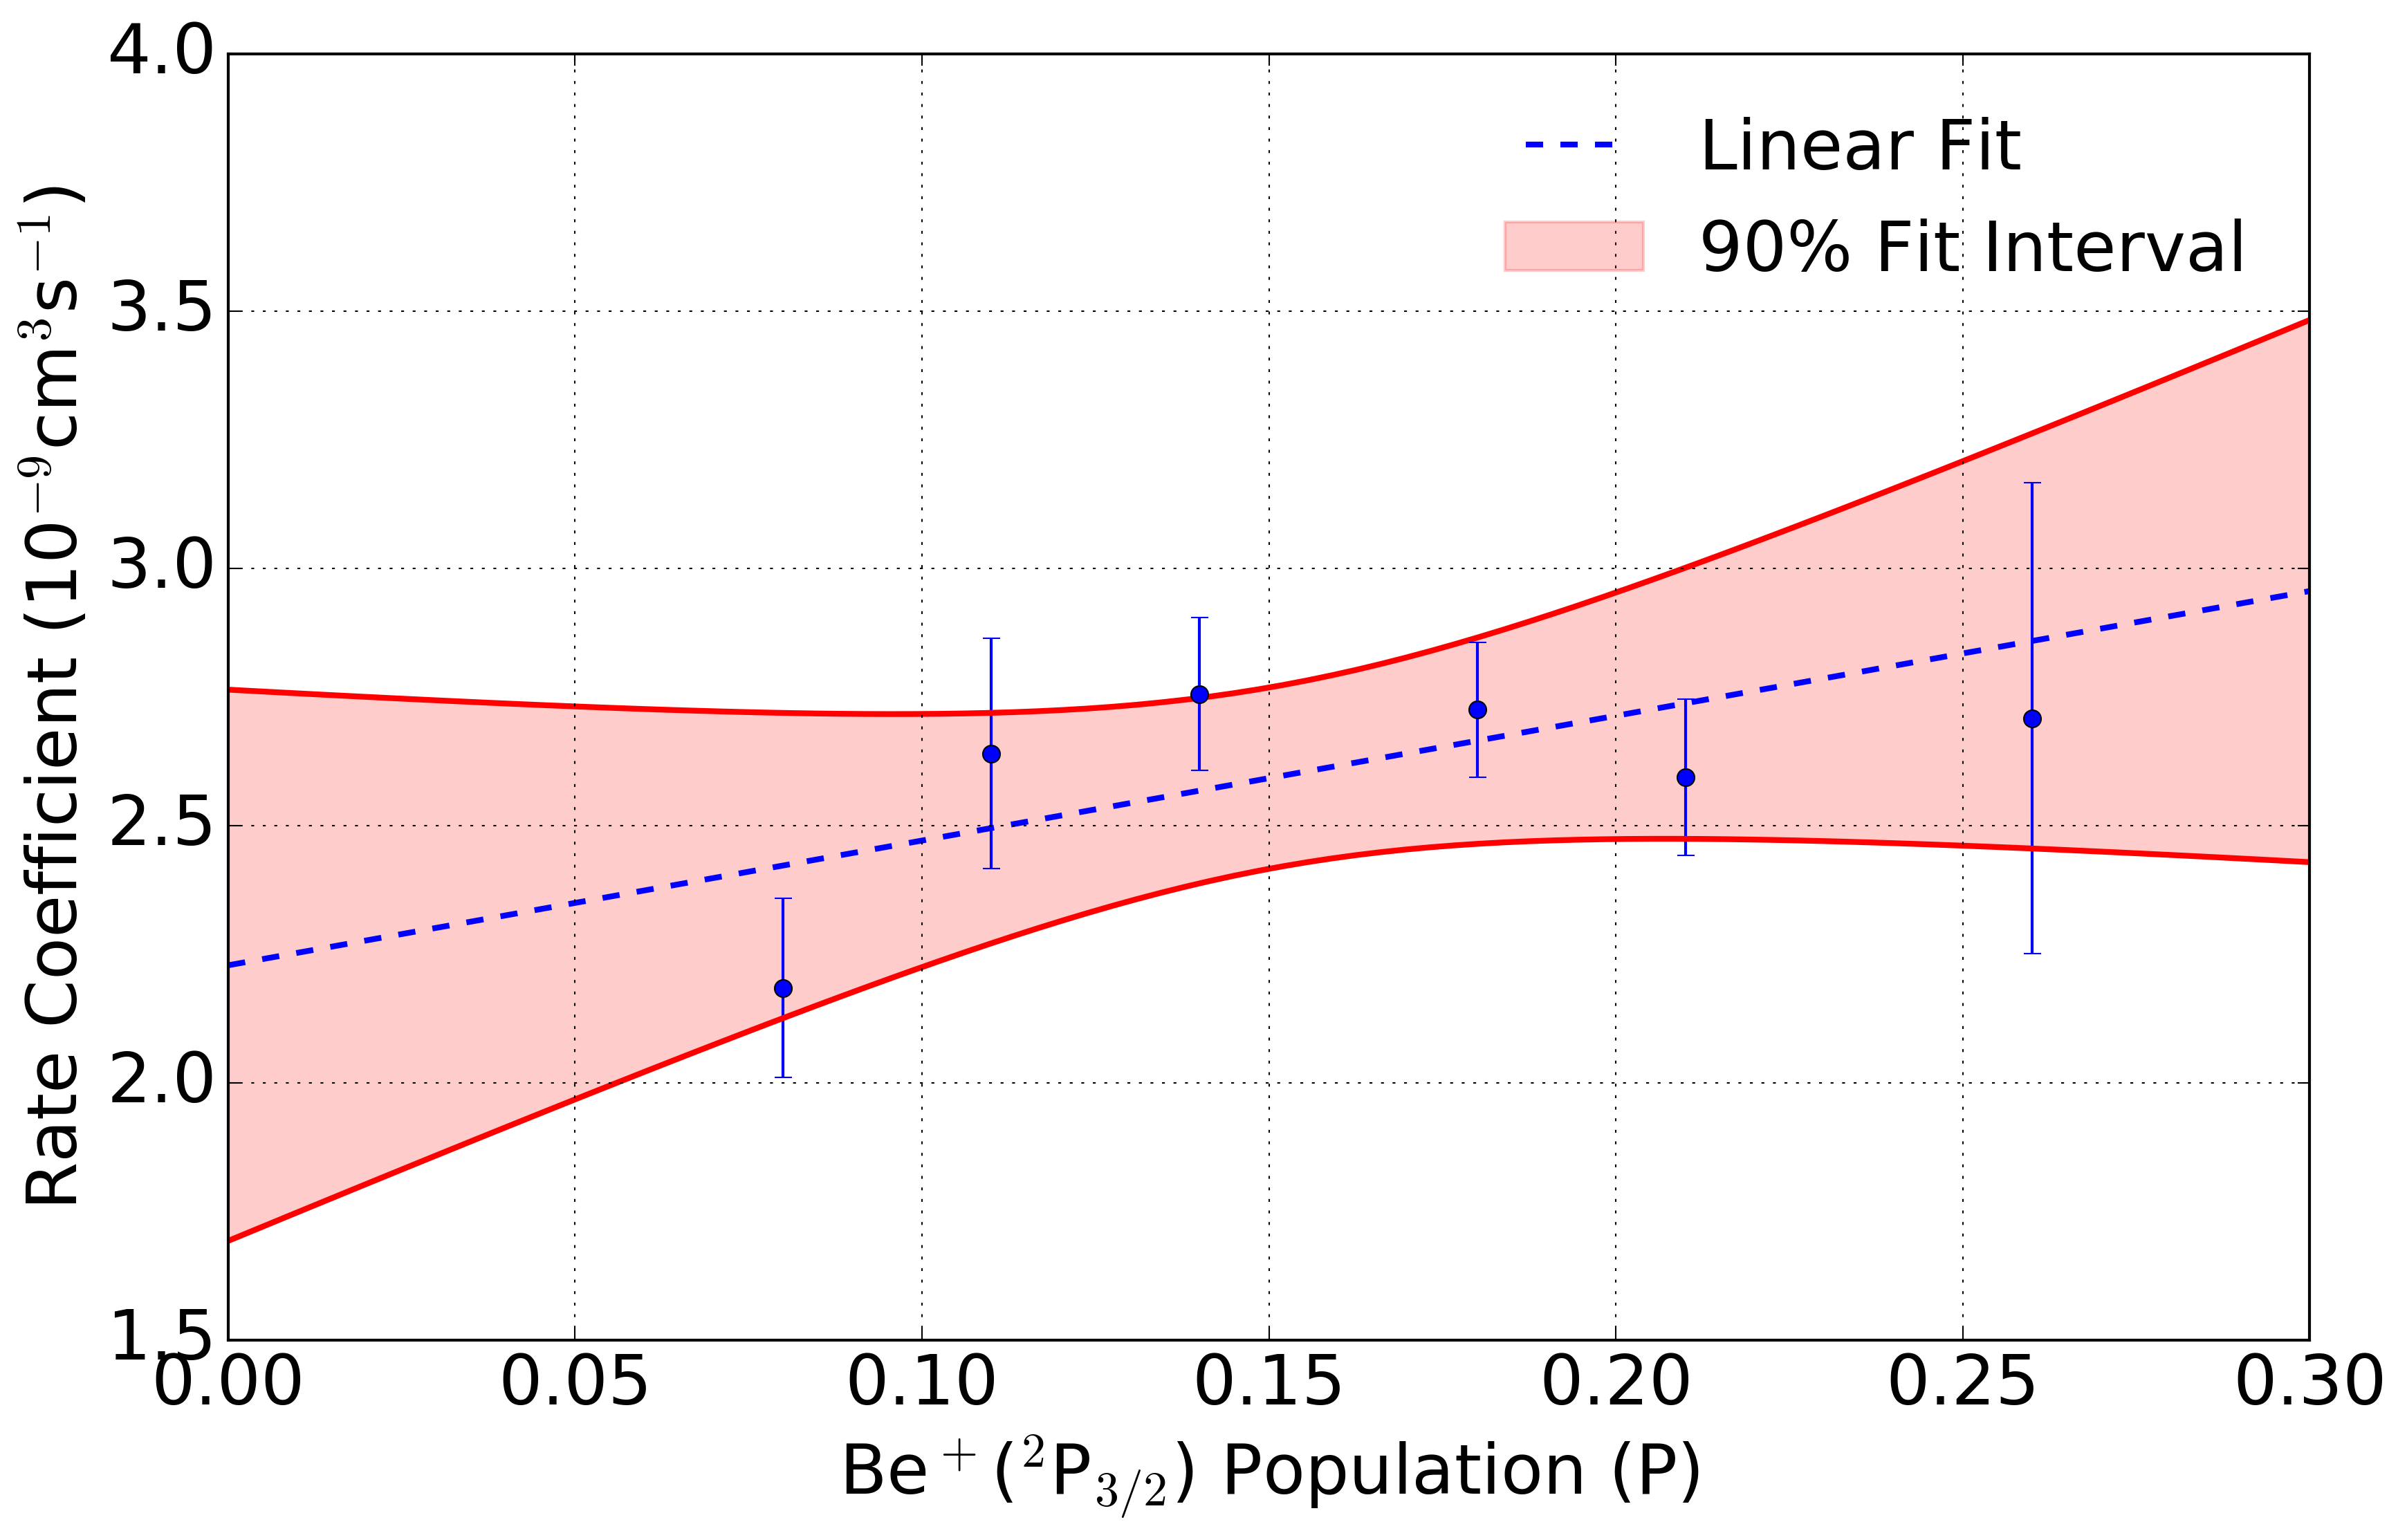
\includegraphics[width=0.8\textwidth]{images/Be_H2O_p_state.png}
	\caption{}
	\label{fig: Be+H2O P-state}
\end{figure}

\begin{figure}
	\centering
	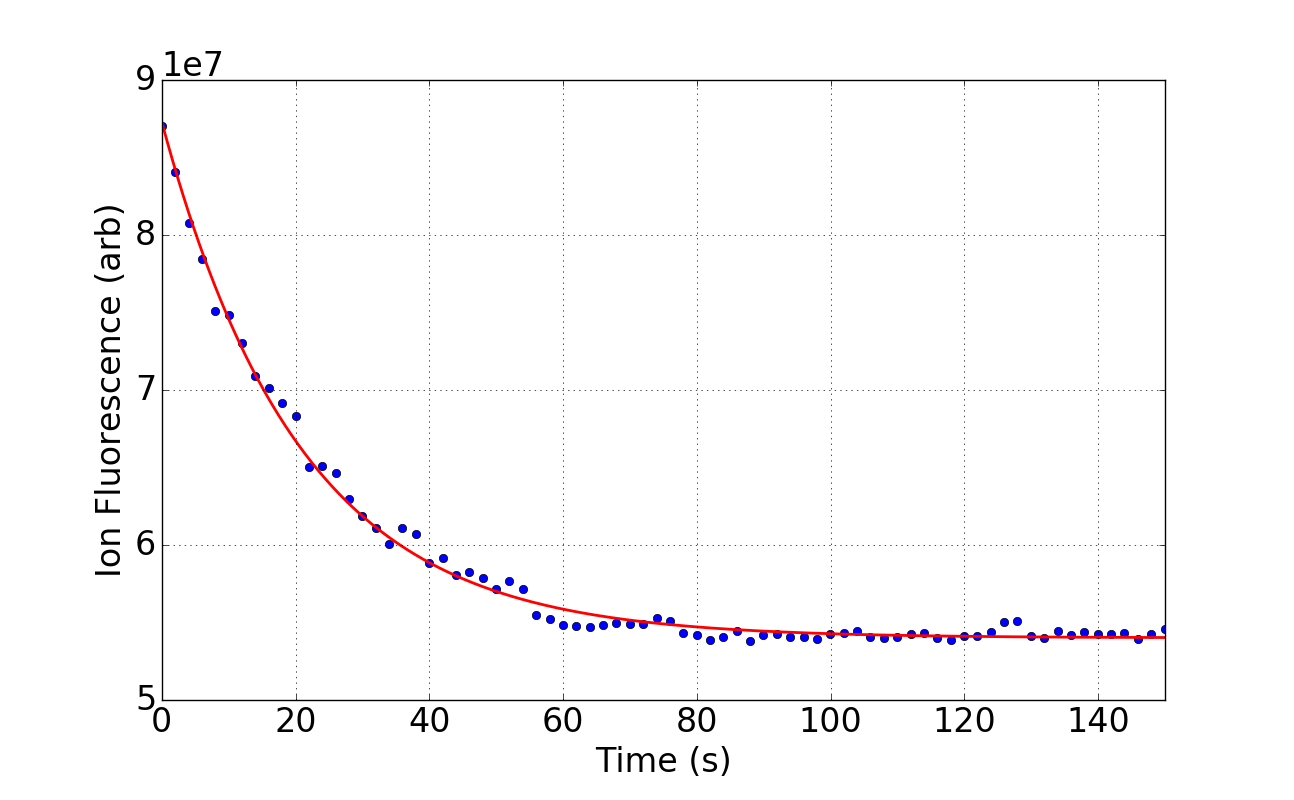
\includegraphics[width=0.8\textwidth]{images/Be_H2O_fluorescence.png}
	\caption{}
	\label{fig: Be+H2O fluorescence}
\end{figure}